\documentclass[a4paper, 12pt]{article}
%%%%%%%%%%%%%%%%%%%%%%%%%%%%%%%%%%%%%%%%%%%%%%%%%%%%%%%%%%%%%%%%%%%%%%%%%%%%%%%
%                                Basic Packages                               %
%%%%%%%%%%%%%%%%%%%%%%%%%%%%%%%%%%%%%%%%%%%%%%%%%%%%%%%%%%%%%%%%%%%%%%%%%%%%%%%

% Gives us multiple colors.
\usepackage[usenames,dvipsnames,pdftex]{xcolor}
% Lets us style link colors.
\usepackage{hyperref}
% Lets us import images and graphics.
\usepackage{graphicx}
% Lets us use figures in floating environments.
\usepackage{float}
% Lets us create multiple columns.
\usepackage{multicol}
% Gives us better math syntax.
\usepackage{amsmath,amsfonts,mathtools,amsthm,amssymb}
% Lets us strikethrough text.
\usepackage{cancel}
% Lets us edit the caption of a figure.
\usepackage{caption}
% Lets us import pdf directly in our tex code.
\usepackage{pdfpages}
% Lets us do algorithm stuff.
\usepackage[ruled,vlined,linesnumbered]{algorithm2e}
% Use a smiley face for our qed symbol.
\usepackage{tikzsymbols}
% \usepackage{fullpage} %%smaller margins
\usepackage[shortlabels]{enumitem}

\setlist[enumerate]{font={\bfseries}} % global settings, for all lists

\usepackage{setspace}
\usepackage[margin=1in, headsep=12pt]{geometry}
\usepackage{wrapfig}
\usepackage{listings}
\usepackage{parskip}

\definecolor{codegreen}{rgb}{0,0.6,0}
\definecolor{codegray}{rgb}{0.5,0.5,0.5}
\definecolor{codepurple}{rgb}{0.58,0,0.82}
\definecolor{backcolour}{rgb}{0.95,0.95,0.95}

\lstdefinestyle{mystyle}{
    backgroundcolor=\color{backcolour},   
    commentstyle=\color{codegreen},
    keywordstyle=\color{magenta},
    numberstyle=\tiny\color{codegray},
    stringstyle=\color{codepurple},
    basicstyle=\ttfamily\footnotesize,
    breakatwhitespace=false,         
    breaklines=true,                 
    captionpos=b,                    
    keepspaces=true,                 
    numbers=left,                    
    numbersep=5pt,                  
    showspaces=false,                
    showstringspaces=false,
    showtabs=false,                  
    tabsize=2,
    numbers=none
}

\lstset{style=mystyle}
\def\class{article}


%%%%%%%%%%%%%%%%%%%%%%%%%%%%%%%%%%%%%%%%%%%%%%%%%%%%%%%%%%%%%%%%%%%%%%%%%%%%%%%
%                                Basic Settings                               %
%%%%%%%%%%%%%%%%%%%%%%%%%%%%%%%%%%%%%%%%%%%%%%%%%%%%%%%%%%%%%%%%%%%%%%%%%%%%%%%

%%%%%%%%%%%%%
%  Symbols  %
%%%%%%%%%%%%%

\let\implies\Rightarrow
\let\impliedby\Leftarrow
\let\iff\Leftrightarrow
\let\epsilon\varepsilon
%%%%%%%%%%%%
%  Tables  %
%%%%%%%%%%%%

\setlength{\tabcolsep}{5pt}
\renewcommand\arraystretch{1.5}

%%%%%%%%%%%%%%
%  SI Unitx  %
%%%%%%%%%%%%%%

\usepackage{siunitx}
\sisetup{locale = FR}

%%%%%%%%%%
%  TikZ  %
%%%%%%%%%%

\usepackage[framemethod=TikZ]{mdframed}
\usepackage{tikz}
\usepackage{tikz-cd}
\usepackage{tikzsymbols}

\usetikzlibrary{intersections, angles, quotes, calc, positioning}
\usetikzlibrary{arrows.meta}

\tikzset{
    force/.style={thick, {Circle[length=2pt]}-stealth, shorten <=-1pt}
}

%%%%%%%%%%%%%%%
%  PGF Plots  %
%%%%%%%%%%%%%%%

\usepackage{pgfplots}
\pgfplotsset{width=10cm, compat=newest}

%%%%%%%%%%%%%%%%%%%%%%%
%  Center Title Page  %
%%%%%%%%%%%%%%%%%%%%%%%

\usepackage{titling}
\renewcommand\maketitlehooka{\null\mbox{}\vfill}
\renewcommand\maketitlehookd{\vfill\null}

%%%%%%%%%%%%%%%%%%%%%%%%%%%%%%%%%%%%%%%%%%%%%%%%%%%%%%%
%  Create a grey background in the middle of the PDF  %
%%%%%%%%%%%%%%%%%%%%%%%%%%%%%%%%%%%%%%%%%%%%%%%%%%%%%%%

\usepackage{eso-pic}
\newcommand\definegraybackground{
    \definecolor{reallylightgray}{HTML}{FAFAFA}
    \AddToShipoutPicture{
        \ifthenelse{\isodd{\thepage}}{
            \AtPageLowerLeft{
                \put(\LenToUnit{\dimexpr\paperwidth-222pt},0){
                    \color{reallylightgray}\rule{222pt}{297mm}
                }
            }
        }
        {
            \AtPageLowerLeft{
                \color{reallylightgray}\rule{222pt}{297mm}
            }
        }
    }
}

%%%%%%%%%%%%%%%%%%%%%%%%
%  Modify Links Color  %
%%%%%%%%%%%%%%%%%%%%%%%%

\hypersetup{
    % Enable highlighting links.
    colorlinks,
    % Change the color of links to blue.
    urlcolor=blue,
    % Change the color of citations to black.
    citecolor={black},
    % Change the color of url's to blue with some black.
    linkcolor={blue!80!black}
}

%%%%%%%%%%%%%%%%%%
% Fix WrapFigure %
%%%%%%%%%%%%%%%%%%

\newcommand{\wrapfill}{\par\ifnum\value{WF@wrappedlines}>0
        \parskip=0pt
        \addtocounter{WF@wrappedlines}{-1}%
        \null\vspace{\arabic{WF@wrappedlines}\baselineskip}%
        \WFclear
    \fi}

%%%%%%%%%%%%%%%%%
% Multi Columns %
%%%%%%%%%%%%%%%%%

\let\multicolmulticols\multicols
\let\endmulticolmulticols\endmulticols

\RenewDocumentEnvironment{multicols}{mO{}}
{%
    \ifnum#1=1
        #2%
    \else % More than 1 column
        \multicolmulticols{#1}[#2]
    \fi
}
{%
    \ifnum#1=1
    \else % More than 1 column
        \endmulticolmulticols
    \fi
}

\newlength{\thickarrayrulewidth}
\setlength{\thickarrayrulewidth}{5\arrayrulewidth}


%%%%%%%%%%%%%%%%%%%%%%%%%%%%%%%%%%%%%%%%%%%%%%%%%%%%%%%%%%%%%%%%%%%%%%%%%%%%%%%
%                           School Specific Commands                          %
%%%%%%%%%%%%%%%%%%%%%%%%%%%%%%%%%%%%%%%%%%%%%%%%%%%%%%%%%%%%%%%%%%%%%%%%%%%%%%%

%%%%%%%%%%%%%%%%%%%%%%%%%%%
%  Initiate New Counters  %
%%%%%%%%%%%%%%%%%%%%%%%%%%%

\newcounter{lecturecounter}

%%%%%%%%%%%%%%%%%%%%%%%%%%
%  Helpful New Commands  %
%%%%%%%%%%%%%%%%%%%%%%%%%%

\makeatletter

\newcommand\resetcounters{
    % Reset the counters for subsection, subsubsection and the definition
    % all the custom environments.
    \setcounter{subsection}{0}
    \setcounter{subsubsection}{0}
    \setcounter{definition0}{0}
    \setcounter{paragraph}{0}
    \setcounter{theorem}{0}
    \setcounter{claim}{0}
    \setcounter{corollary}{0}
    \setcounter{proposition}{0}
    \setcounter{lemma}{0}
    \setcounter{exercise}{0}
    \setcounter{problem}{0}
    
    \setcounter{subparagraph}{0}
    % \@ifclasswith\class{nocolor}{
    %     \setcounter{definition}{0}
    % }{}
}

%%%%%%%%%%%%%%%%%%%%%
%  Lecture Command  %
%%%%%%%%%%%%%%%%%%%%%

\usepackage{xifthen}

% EXAMPLE:
% 1. \lecture{Oct 17 2022 Mon (08:46:48)}{Lecture Title}
% 2. \lecture[4]{Oct 17 2022 Mon (08:46:48)}{Lecture Title}
% 3. \lecture{Oct 17 2022 Mon (08:46:48)}{}
% 4. \lecture[4]{Oct 17 2022 Mon (08:46:48)}{}
% Parameters:
% 1. (Optional) lecture number.
% 2. Time and date of lecture.
% 3. Lecture Title.
\def\@lecture{}
\def\@lectitle{}
\def\@leccount{}
\newcommand\lecture[3]{
    \newpage

    % Check if user passed the lecture title or not.
    \def\@leccount{Lecture #1}
    \ifthenelse{\isempty{#3}}{
        \def\@lecture{Lecture #1}
        \def\@lectitle{Lecture #1}
    }{
        \def\@lecture{Lecture #1: #3}
        \def\@lectitle{#3}
    }

    \setcounter{section}{#1}
    \renewcommand\thesubsection{#1.\arabic{subsection}}
    
    \phantomsection
    \addcontentsline{toc}{section}{\@lecture}
    \resetcounters

    \begin{mdframed}
        \begin{center}
            \Large \textbf{\@leccount}
            
            \vspace*{0.2cm}
            
            \large \@lectitle
            
            
            \vspace*{0.2cm}

            \normalsize #2
        \end{center}
    \end{mdframed}

}

%%%%%%%%%%%%%%%%%%%%
%  Import Figures  %
%%%%%%%%%%%%%%%%%%%%

\usepackage{import}
\pdfminorversion=7

% EXAMPLE:
% 1. \incfig{limit-graph}
% 2. \incfig[0.4]{limit-graph}
% Parameters:
% 1. The figure name. It should be located in figures/NAME.tex_pdf.
% 2. (Optional) The width of the figure. Example: 0.5, 0.35.
\newcommand\incfig[2][1]{%
    \def\svgwidth{#1\columnwidth}
    \import{./figures/}{#2.pdf_tex}
}

\begingroup\expandafter\expandafter\expandafter\endgroup
\expandafter\ifx\csname pdfsuppresswarningpagegroup\endcsname\relax
\else
    \pdfsuppresswarningpagegroup=1\relax
\fi

%%%%%%%%%%%%%%%%%
% Fancy Headers %
%%%%%%%%%%%%%%%%%

\usepackage{fancyhdr}

% Force a new page.
\newcommand\forcenewpage{\clearpage\mbox{~}\clearpage\newpage}

% This command makes it easier to manage my headers and footers.
\newcommand\createintro{
    % Use roman page numbers (e.g. i, v, vi, x, ...)
    \pagenumbering{roman}

    % Display the page style.
    \maketitle
    % Make the title pagestyle empty, meaning no fancy headers and footers.
    \thispagestyle{empty}
    % Create a newpage.
    \newpage

    % Input the intro.tex page if it exists.
    \IfFileExists{intro.tex}{ % If the intro.tex file exists.
        % Input the intro.tex file.
        \textbf{Course}: MATH 16300: Honors Calculus III

\textbf{Section}: 43

\textbf{Professor}: Minjae Park

\textbf{At}: The University of Chicago

\textbf{Quarter}: Spring 2023

\textbf{Course materials}: Calculus by Spivak (4th Edition), Calculus On Manifolds by Spivak

\vspace{1cm}
\textbf{Disclaimer}: This document will inevitably contain some mistakes, both simple typos and serious logical and mathematical errors. Take what you read with a grain of salt as it is made by an undergraduate student going through the learning process himself. If you do find any error, I would really appreciate it if you can let me know by email at \href{mailto:conghungletran@gmail.com}{conghungletran@gmail.com}.

        % Make the pagestyle fancy for the intro.tex page.
        \pagestyle{fancy}

        % Remove the line for the header.
        \renewcommand\headrulewidth{0pt}

        % Remove all header stuff.
        \fancyhead{}

        % Add stuff for the footer in the center.
        % \fancyfoot[C]{
        %   \textit{For more notes like this, visit
        %   \href{\linktootherpages}{\shortlinkname}}. \\
        %   \vspace{0.1cm}
        %   \hrule
        %   \vspace{0.1cm}
        %   \@author, \\
        %   \term: \academicyear, \\
        %   Last Update: \@date, \\
        %   \faculty
        % }

        \newpage
    }{ % If the intro.tex file doesn't exist.
        % Force a \newpageage.
        % \forcenewpage
        \newpage
    }

    % Remove the center stuff we did above, and replace it with just the page
    % number, which is still in roman numerals.
    \fancyfoot[C]{\thepage}
    % Add the table of contents.
    \tableofcontents
    % Force a new page.
    \newpage

    % Move the page numberings back to arabic, from roman numerals.
    \pagenumbering{arabic}
    % Set the page number to 1.
    \setcounter{page}{1}

    % Add the header line back.
    \renewcommand\headrulewidth{0.4pt}
    % In the top right, add the lecture title.
    \fancyhead[R]{\footnotesize \@lecture}
    % In the top left, add the author name.
    \fancyhead[L]{\footnotesize \@author}
    % In the bottom center, add the page.
    \fancyfoot[C]{\thepage}
    % Add a nice gray background in the middle of all the upcoming pages.
    % \definegraybackground
}

\makeatother


%%%%%%%%%%%%%%%%%%%%%%%%%%%%%%%%%%%%%%%%%%%%%%%%%%%%%%%%%%%%%%%%%%%%%%%%%%%%%%%
%                               Custom Commands                               %
%%%%%%%%%%%%%%%%%%%%%%%%%%%%%%%%%%%%%%%%%%%%%%%%%%%%%%%%%%%%%%%%%%%%%%%%%%%%%%%

%%%%%%%%%%%%
%  Circle  %
%%%%%%%%%%%%

\newcommand*\circled[1]{\tikz[baseline= (char.base)]{
        \node[shape=circle,draw,inner sep=1pt] (char) {#1};}
}

%%%%%%%%%%%%%%%%%%%
%  Todo Commands  %
%%%%%%%%%%%%%%%%%%%

% \usepackage{xargs}
% \usepackage[colorinlistoftodos]{todonotes}

% \makeatletter

% \@ifclasswith\class{working}{
%     \newcommandx\unsure[2][1=]{\todo[linecolor=red,backgroundcolor=red!25,bordercolor=red,#1]{#2}}
%     \newcommandx\change[2][1=]{\todo[linecolor=blue,backgroundcolor=blue!25,bordercolor=blue,#1]{#2}}
%     \newcommandx\info[2][1=]{\todo[linecolor=OliveGreen,backgroundcolor=OliveGreen!25,bordercolor=OliveGreen,#1]{#2}}
%     \newcommandx\improvement[2][1=]{\todo[linecolor=Plum,backgroundcolor=Plum!25,bordercolor=Plum,#1]{#2}}

%     \newcommand\listnotes{
%         \newpage
%         \listoftodos[Notes]
%     }
% }{
%     \newcommandx\unsure[2][1=]{}
%     \newcommandx\change[2][1=]{}
%     \newcommandx\info[2][1=]{}
%     \newcommandx\improvement[2][1=]{}

%     \newcommand\listnotes{}
% }

% \makeatother

%%%%%%%%%%%%%
%  Correct  %
%%%%%%%%%%%%%

% EXAMPLE:
% 1. \correct{INCORRECT}{CORRECT}
% Parameters:
% 1. The incorrect statement.
% 2. The correct statement.
\definecolor{correct}{HTML}{009900}
\newcommand\correct[2]{{\color{red}{#1 }}\ensuremath{\to}{\color{correct}{ #2}}}


%%%%%%%%%%%%%%%%%%%%%%%%%%%%%%%%%%%%%%%%%%%%%%%%%%%%%%%%%%%%%%%%%%%%%%%%%%%%%%%
%                                 Environments                                %
%%%%%%%%%%%%%%%%%%%%%%%%%%%%%%%%%%%%%%%%%%%%%%%%%%%%%%%%%%%%%%%%%%%%%%%%%%%%%%%

\usepackage{varwidth}
\usepackage{thmtools}
\usepackage[most,many,breakable]{tcolorbox}

\tcbuselibrary{theorems,skins,hooks}
\usetikzlibrary{arrows,calc,shadows.blur}

%%%%%%%%%%%%%%%%%%%
%  Define Colors  %
%%%%%%%%%%%%%%%%%%%

% color prototype
% \definecolor{color}{RGB}{45, 111, 177}

% ESSENTIALS: 
\definecolor{myred}{HTML}{c74540}
\definecolor{myblue}{HTML}{072b85}
\definecolor{mygreen}{HTML}{388c46}
\definecolor{myblack}{HTML}{000000}

\colorlet{definition_color}{myred}

\colorlet{theorem_color}{myblue}
\colorlet{lemma_color}{myblue}
\colorlet{prop_color}{myblue}
\colorlet{corollary_color}{myblue}
\colorlet{claim_color}{myblue}

\colorlet{proof_color}{myblack}
\colorlet{example_color}{myblack}
\colorlet{exercise_color}{myblack}

% MISCS: 
%%%%%%%%%%%%%%%%%%%%%%%%%%%%%%%%%%%%%%%%%%%%%%%%%%%%%%%%%
%  Create Environments Styles Based on Given Parameter  %
%%%%%%%%%%%%%%%%%%%%%%%%%%%%%%%%%%%%%%%%%%%%%%%%%%%%%%%%%

% \mdfsetup{skipabove=1em,skipbelow=0em}

%%%%%%%%%%%%%%%%%%%%%%
%  Helpful Commands  %
%%%%%%%%%%%%%%%%%%%%%%

% EXAMPLE:
% 1. \createnewtheoremstyle{thmdefinitionbox}{}{}
% 2. \createnewtheoremstyle{thmtheorembox}{}{}
% 3. \createnewtheoremstyle{thmproofbox}{qed=\qedsymbol}{
%       rightline=false, topline=false, bottomline=false
%    }
% Parameters:
% 1. Theorem name.
% 2. Any extra parameters to pass directly to declaretheoremstyle.
% 3. Any extra parameters to pass directly to mdframed.
\newcommand\createnewtheoremstyle[3]{
    \declaretheoremstyle[
        headfont=\bfseries\sffamily, bodyfont=\normalfont, #2,
        mdframed={
                #3,
            },
    ]{#1}
}

% EXAMPLE:
% 1. \createnewcoloredtheoremstyle{thmdefinitionbox}{definition}{}{}
% 2. \createnewcoloredtheoremstyle{thmexamplebox}{example}{}{
%       rightline=true, leftline=true, topline=true, bottomline=true
%     }
% 3. \createnewcoloredtheoremstyle{thmproofbox}{proof}{qed=\qedsymbol}{backgroundcolor=white}
% Parameters:
% 1. Theorem name.
% 2. Color of theorem.
% 3. Any extra parameters to pass directly to declaretheoremstyle.
% 4. Any extra parameters to pass directly to mdframed.

% change backgroundcolor to #2!5 if user wants a colored backdrop to theorem environments. It's a cool color theme, but there's too much going on in the page.
\newcommand\createnewcoloredtheoremstyle[4]{
    \declaretheoremstyle[
        headfont=\bfseries\sffamily\color{#2},
        bodyfont=\normalfont,
        headpunct=,
        headformat = \NAME~\NUMBER\NOTE \hfill\smallskip\linebreak,
        #3,
        mdframed={
                outerlinewidth=0.75pt,
                rightline=false,
                leftline=false,
                topline=false,
                bottomline=false,
                backgroundcolor=white,
                skipabove = 5pt,
                skipbelow = 0pt,
                linecolor=#2,
                innertopmargin = 0pt,
                innerbottommargin = 0pt,
                innerrightmargin = 4pt,
                innerleftmargin= 6pt,
                leftmargin = -6pt,
                #4,
            },
    ]{#1}
}



%%%%%%%%%%%%%%%%%%%%%%%%%%%%%%%%%%%
%  Create the Environment Styles  %
%%%%%%%%%%%%%%%%%%%%%%%%%%%%%%%%%%%

\makeatletter
\@ifclasswith\class{nocolor}{
    % Environments without color.

    % ESSENTIALS:
    \createnewtheoremstyle{thmdefinitionbox}{}{}
    \createnewtheoremstyle{thmtheorembox}{}{}
    \createnewtheoremstyle{thmproofbox}{qed=\qedsymbol}{}
    \createnewtheoremstyle{thmcorollarybox}{}{}
    \createnewtheoremstyle{thmlemmabox}{}{}
    \createnewtheoremstyle{thmclaimbox}{}{}
    \createnewtheoremstyle{thmexamplebox}{}{}

    % MISCS: 
    \createnewtheoremstyle{thmpropbox}{}{}
    \createnewtheoremstyle{thmexercisebox}{}{}
    \createnewtheoremstyle{thmexplanationbox}{}{}
    \createnewtheoremstyle{thmremarkbox}{}{}
    
    % STYLIZED MORE BELOW
    \createnewtheoremstyle{thmquestionbox}{}{}
    \createnewtheoremstyle{thmsolutionbox}{qed=\qedsymbol}{}
}{
    % Environments with color.

    % ESSENTIALS: definition, theorem, proof, corollary, lemma, claim, example
    \createnewcoloredtheoremstyle{thmdefinitionbox}{definition_color}{}{leftline=false}
    \createnewcoloredtheoremstyle{thmtheorembox}{theorem_color}{}{leftline=false}
    \createnewcoloredtheoremstyle{thmproofbox}{proof_color}{qed=\qedsymbol}{}
    \createnewcoloredtheoremstyle{thmcorollarybox}{corollary_color}{}{leftline=false}
    \createnewcoloredtheoremstyle{thmlemmabox}{lemma_color}{}{leftline=false}
    \createnewcoloredtheoremstyle{thmpropbox}{prop_color}{}{leftline=false}
    \createnewcoloredtheoremstyle{thmclaimbox}{claim_color}{}{leftline=false}
    \createnewcoloredtheoremstyle{thmexamplebox}{example_color}{}{}
    \createnewcoloredtheoremstyle{thmexplanationbox}{example_color}{qed=\qedsymbol}{}
    \createnewcoloredtheoremstyle{thmremarkbox}{theorem_color}{}{}

    \createnewcoloredtheoremstyle{thmmiscbox}{black}{}{}

    \createnewcoloredtheoremstyle{thmexercisebox}{exercise_color}{}{}
    \createnewcoloredtheoremstyle{thmproblembox}{theorem_color}{}{leftline=false}
    \createnewcoloredtheoremstyle{thmsolutionbox}{mygreen}{qed=\qedsymbol}{}
}
\makeatother

%%%%%%%%%%%%%%%%%%%%%%%%%%%%%
%  Create the Environments  %
%%%%%%%%%%%%%%%%%%%%%%%%%%%%%
\declaretheorem[numberwithin=section, style=thmdefinitionbox,     name=Definition]{definition}
\declaretheorem[numberwithin=section, style=thmtheorembox,     name=Theorem]{theorem}
\declaretheorem[numbered=no,          style=thmexamplebox,     name=Example]{example}
\declaretheorem[numberwithin=section, style=thmtheorembox,       name=Claim]{claim}
\declaretheorem[numberwithin=section, style=thmcorollarybox,   name=Corollary]{corollary}
\declaretheorem[numberwithin=section, style=thmpropbox,        name=Proposition]{proposition}
\declaretheorem[numberwithin=section, style=thmlemmabox,       name=Lemma]{lemma}
\declaretheorem[numberwithin=section, style=thmexercisebox,    name=Exercise]{exercise}
\declaretheorem[numbered=no,          style=thmproofbox,       name=Proof]{proof0}
\declaretheorem[numbered=no,          style=thmexplanationbox, name=Explanation]{explanation}
\declaretheorem[numbered=no,          style=thmsolutionbox,    name=Solution]{solution}
\declaretheorem[numberwithin=section,          style=thmproblembox,     name=Problem]{problem}
\declaretheorem[numbered=no,          style=thmmiscbox,    name=Intuition]{intuition}
\declaretheorem[numbered=no,          style=thmmiscbox,    name=Goal]{goal}
\declaretheorem[numbered=no,          style=thmmiscbox,    name=Recall]{recall}
\declaretheorem[numbered=no,          style=thmmiscbox,    name=Motivation]{motivation}
\declaretheorem[numbered=no,          style=thmmiscbox,    name=Remark]{remark}
\declaretheorem[numbered=no,          style=thmmiscbox,    name=Observe]{observe}
\declaretheorem[numbered=no,          style=thmmiscbox,    name=Question]{question}


%%%%%%%%%%%%%%%%%%%%%%%%%%%%
%  Edit Proof Environment  %
%%%%%%%%%%%%%%%%%%%%%%%%%%%%

\renewenvironment{proof}[2][\proofname]{
    % \vspace{-12pt}
    \begin{proof0} [#2]
        }{\end{proof0}}

\theoremstyle{definition}

\newtheorem*{notation}{Notation}
\newtheorem*{previouslyseen}{As previously seen}
\newtheorem*{property}{Property}
% \newtheorem*{intuition}{Intuition}
% \newtheorem*{goal}{Goal}
% \newtheorem*{recall}{Recall}
% \newtheorem*{motivation}{Motivation}
% \newtheorem*{remark}{Remark}
% \newtheorem*{observe}{Observe}

\author{Hung C. Le Tran}


%%%% MATH SHORTHANDS %%%%
%% blackboard bold math capitals
\DeclareMathOperator*{\esssup}{ess\,sup}
\DeclareMathOperator*{\Hom}{Hom}
\newcommand{\bbf}{\mathbb{F}}
\newcommand{\bbn}{\mathbb{N}}
\newcommand{\bbq}{\mathbb{Q}}
\newcommand{\bbr}{\mathbb{R}}
\newcommand{\bbz}{\mathbb{Z}}
\newcommand{\bbc}{\mathbb{C}}
\newcommand{\bbk}{\mathbb{K}}
\newcommand{\bbm}{\mathbb{M}}
\newcommand{\bbp}{\mathbb{P}}
\newcommand{\bbe}{\mathbb{E}}

\newcommand{\bfw}{\mathbf{w}}
\newcommand{\bfx}{\mathbf{x}}
\newcommand{\bfX}{\mathbf{X}}
\newcommand{\bfy}{\mathbf{y}}
\newcommand{\bfyhat}{\mathbf{\hat{y}}}

\newcommand{\calb}{\mathcal{B}}
\newcommand{\calf}{\mathcal{F}}
\newcommand{\calt}{\mathcal{T}}
\newcommand{\call}{\mathcal{L}}
\renewcommand{\phi}{\varphi}

% Universal Math Shortcuts
\newcommand{\st}{\hspace*{2pt}\text{s.t.}\hspace*{2pt}}
\newcommand{\pffwd}{\hspace*{2pt}\fbox{\(\Rightarrow\)}\hspace*{10pt}}
\newcommand{\pfbwd}{\hspace*{2pt}\fbox{\(\Leftarrow\)}\hspace*{10pt}}
\newcommand{\contra}{\ensuremath{\Rightarrow\Leftarrow}}
\newcommand{\cvgn}{\xrightarrow{n \to \infty}}
\newcommand{\cvgj}{\xrightarrow{j \to \infty}}

\newcommand{\im}{\mathrm{im}}
\newcommand{\innerproduct}[2]{\langle #1, #2 \rangle}
\newcommand*{\conj}[1]{\overline{#1}}

% https://tex.stackexchange.com/questions/438612/space-between-exists-and-forall
% https://tex.stackexchange.com/questions/22798/nice-looking-empty-set
\let\oldforall\forall
\renewcommand{\forall}{\;\oldforall\; }
\let\oldexist\exists
\renewcommand{\exists}{\;\oldexist\; }
\newcommand\existu{\;\oldexist!\: }
\let\oldemptyset\emptyset
\let\emptyset\varnothing


\renewcommand{\_}[1]{\underline{#1}}
\DeclarePairedDelimiter{\abs}{\lvert}{\rvert}
\DeclarePairedDelimiter{\norm}{\lVert}{\rVert}
\DeclarePairedDelimiter\ceil{\lceil}{\rceil}
\DeclarePairedDelimiter\floor{\lfloor}{\rfloor}
\setlength\parindent{0pt}
\setlength{\headheight}{12.0pt}
\addtolength{\topmargin}{-12.0pt}


% Default skipping, change if you want more spacing
% \thinmuskip=3mu
% \medmuskip=4mu plus 2mu minus 4mu
% \thickmuskip=5mu plus 5mu

% \DeclareMathOperator{\ext}{ext}
% \DeclareMathOperator{\bridge}{bridge}
\title{CMSC 25300: Mathematical Foundations of ML \\ \large Problem Set 5}
\date{11 Nov 2023}
\author{Hung Le Tran}
\begin{document}
\maketitle
\setcounter{section}{5}
\begin{problem} [Problem 1]
\end{problem}
\begin{solution}
    \textbf{(a)}
    \begin{align*}
        \bfX        & = \bfU \bfSigma \bfV^T                              \\
        \bfX        & = \sum_{i=1}^{k}\bfu_i \sigma_i \bfv_i^T            \\
        \bfX^T      & = (\bfU \bfSigma \bfV^T)^T = \bfV \bfSigma^T \bfU^T \\
        \bfX \bfX^T & = (\bfU \bfSigma \bfV^T)(\bfV \bfSigma^T \bfU^T )   \\
                    & = \bfU (\bfSigma \bfSigma^T) \bfU^T                 \\
        \bfX^T \bfX & = (\bfV \bfSigma^T \bfU^T )(\bfU \bfSigma \bfV^T)   \\
                    & = \bfV (\bfSigma^T \bfSigma) \bfV^T
    \end{align*}

    \textbf{(b)(i)}
    \[
        \bfX = \begin{bmatrix}
            3 & 0 & 0 & 0 \\
            0 & 1 & 0 & 0 \\
            0 & 0 & 0 & 0 \\
            0 & 0 & 0 & 0
        \end{bmatrix}, \bfy = \begin{bmatrix}
            6 \\ 2 \\ 1 \\ 2
        \end{bmatrix}
    \]

    The squared error is minimized when

    \begin{align*}
        \bfX^T \bfy     & = \bfX^T \bfX \bfw \\
        \begin{bmatrix}
            18 \\
            2  \\
            0  \\
            0
        \end{bmatrix} & = \begin{bmatrix}
                              9 & 0 & 0 & 0 \\
                              0 & 1 & 0 & 0 \\
                              0 & 0 & 0 & 0 \\
                              0 & 0 & 0 & 0
                          \end{bmatrix} \bfw
    \end{align*}
    so \[
        18 = 9\bfw_1, 2 = w_2 \implies \bfw_1 = \bfw_2 = 2
    \]
    Therefore the set of $\bfw$ that minimizes the squared error is \[
        W = \left\{\begin{bmatrix}
            2 \\2\\a\\b
        \end{bmatrix} : a, b \in \bbr\right\}
    \]

    Clearly, the one with the smallest norm has $a = b = 0$, i.e. \[
        \hat{\bfw} = \begin{bmatrix}
            2 \\2 \\ 0 \\0
        \end{bmatrix}
    \]

    \textbf{(b)(ii)}

    \[\bfX = \bfU \bfSigma \bfV^T\]

    The $(n-k+1)$ last right singular vectors, i.e., $\bfv_{k+1}, \bfv_{k+2}, \dots, \bfv_n$ form a basis for the null space of $\bfX$.

    We have:
    \begin{align*}
        \bfX \bfw & = \sum_{i=1}^{k} \bfu_i \sigma_i \bfv_i^T \bfw   \\
                  & = \sum_{i=1}^{k} \bfu_i \sigma_i (\bfv_i^T \bfw)
    \end{align*}

    Notice that if for any $i$, $\bfv_i^T \bfw$ is non-zero, then since $\{\bfu_i\}$ are linearly independent, $\bfX \bfw$ would then be non-zero.

    Therefore $\bfv_i^T \bfw = 0 \forall 1 \leq i \leq k$. The basis of the space of $\bfw$ that satisfies this is $\{\bfv_{k+1}, \bfv_{k+2}, \dots, \bfv_n\}$, since $\{\bfv_i\}$ are orthonormal vectors.

    \textbf{(b)(iii)}
    \begin{align*}
        \norm{\tilde{\bfy} - \bfSigma \tilde{\bfw}}^2 & = \tilde{\bfy}^T \tilde{\bfy} - 2 \tilde{\bfy}^T \bfSigma \tilde{\bfw} + \tilde{\bfw}^T \bfSigma^T \bfSigma \tilde{\bfw} \\
                                                      & = \bfy^T \bfU^T \bfU \bfy - 2 \bfy^T \bfU \bfSigma \bfV^T \bfw + \bfw^T \bfV \bfSigma^T \bfSigma \bfV^T \bfw             \\
                                                      & = \bfy^T \bfy - 2\bfy^T \bfX \bfw + \bfw^T \bfV \bfSigma^T \bfU^T \bfU \bfSigma \bfV^T \bfw                              \\
                                                      & = \bfy^T \bfy - 2 \bfy^T \bfX \bfw + (\bfX \bfw)^T (\bfX \bfw)                                                           \\
                                                      & = \norm{\bfy - \bfX \bfw}^2
    \end{align*}

    Therefore the set of $\tilde{\bfw}$ that minimizes the norm above is \[
        A = \left\{\bfV^T \begin{bmatrix}
            2 \\2 \\ a \\b
        \end{bmatrix}: a, b \in \bbr\right\}
    \]
    The SVD of our particular $X$ is \[
        \bfX = I \begin{bmatrix}
            3 & 0 & 0 & 0 \\
            0 & 1 & 0 & 0 \\
            0 & 0 & 0 & 0 \\
            0 & 0 & 0 & 0
        \end{bmatrix}I
    \]
    so \[
        A = \left\{I\begin{bmatrix}
            2 \\2 \\ a \\b
        \end{bmatrix}: a, b \in \bbr\right\} = \left\{\begin{bmatrix}
            2 \\2 \\ a \\b
        \end{bmatrix}: a, b \in \bbr\right\}
    \]

    the one with the smallest norm is $\begin{bmatrix}
            2 \\2 \\ 0 \\0
        \end{bmatrix}$

    \textbf{(b)(iv)} Given \[
    \tilde{\bfw} = \begin{bmatrix}
    2 \\2 \\
    0\\
    0
    \end{bmatrix}
    \]
    \[
    \bfw = I^{-1}\tilde{\bfw} = \begin{bmatrix}
        2 \\2 \\ 0 \\0
    \end{bmatrix}
    \]

    \textbf{(c)}
\begin{lstlisting} [language=python]
import numpy as np

import matplotlib.pyplot as plt

data = np.load("blurring.npz")
X = data['X']
y = data['y']

U, S, Vt = np.linalg.svd(X, full_matrices=False)

V = Vt.T
Sm = np.diag(S)
w_LS = V @ np.linalg.inv(Sm.T @ Sm) @ Sm.T @ U.T @ y

Spseudo = (S > 0) * (1/S)

w_15 = V[:, :15] @ np.diag(Spseudo[:15]) @ U[:, :15].T @ y
w_75 = V[:, :75] @ np.diag(Spseudo[:75]) @ U[:, :75].T @ y
w_150 = V[:, :150] @ np.diag(Spseudo[:150]) @ U[:, :150].T @ y

plt.plot(data['w'], label='true w')
plt.plot(w_LS, alpha=0.7, c='red', label='LS estimate')
plt.legend()
plt.show()

plt.plot(data['w'], label = 'true w')
plt.plot(w_15, alpha=0.7, c='red', label = 'k=15')
plt.plot(w_75, alpha=0.7, c='orange', label = 'k=75')
plt.plot(w_150, alpha=0.7, c='purple', label = 'k=150')

plt.legend()
plt.show()

print(np.linalg.norm(w_LS - data['w']))
print(np.linalg.norm(w_15 - data['w']))
print(np.linalg.norm(w_75 - data['w']))
print(np.linalg.norm(w_150 - data['w']))    
\end{lstlisting}
which prints 
\begin{lstlisting}
14.840043525210662
12.003106141836785
6.390503358052758
5.102851020292181
\end{lstlisting}
and following plots:
    \begin{center}
    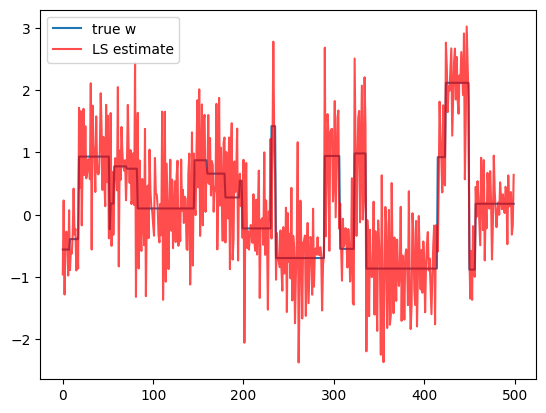
\includegraphics[width=8cm]{./figures/5.1c.1.png}
    \end{center}
    \begin{center}
    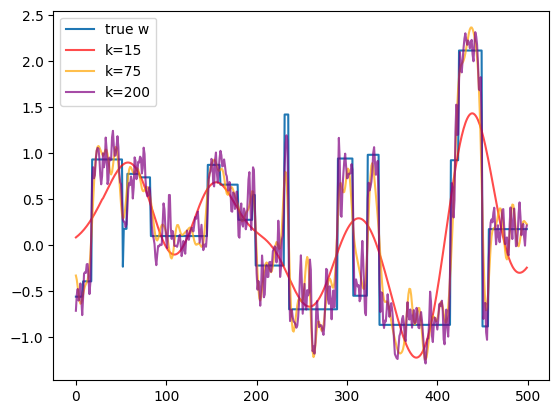
\includegraphics[width=8cm]{./figures/5.1c.2.png}
    \end{center}

    \textbf{(i), (ii)} The impact of the added noise is tremendous in the least squares estimation, with high variance in small time increments.

    The code printed the following 2-norm between $\bfw_{LS}$ and true $\bfw$: 14.840043525210662, which is relatively high when compared to the approximations produced by truncated SVD: 12.003106141836785, 6.390503358052758, 5.102851020292181 respectively. The higher values of $k$ produced better approximates for the true value of $\bfw$, as seen in the red line for $k=15$, there wasn't much variation and flexibility, while for $k = 200$, the purple line showed more flexibility and tracked the true value of $\bfw$ more closely.
\end{solution}

\begin{problem} [Problem 2]
\end{problem}
\begin{solution}
    \textbf{(a)} 
    \[
    M = \begin{bmatrix}
    0 & 0 & 0 & 1 \\
    1 & 0 & 0 & 0 \\
    0 & 1 & 0 & 0 \\
    0 & 1 & 1 & 0
    \end{bmatrix}
    \]
    and \[
    A =  \begin{bmatrix}
        0 & 0 & 0 & 1 \\
        1 & 0 & 0 & 0 \\
        0 & 1/2 & 0 & 0 \\
        0 & 1/2 & 1 & 0
        \end{bmatrix}
    \]

    \textbf{(b)}    

\begin{lstlisting} [language=python]
pi = np.array([0.25, 0.25, 0.25, 0.25])

A = np.array([0, 0, 0, 1, 1, 0 , 0, 0, 0, 0.5, 0, 0, 0, 0.5, 1, 0]).reshape((4, 4))

for i in range(10000):
    pi = A @ pi
print(pi)
\end{lstlisting}
    which prints
\begin{lstlisting}
[0.28571429 0.28571429 0.14285714 0.28571429]
\end{lstlisting}

\textbf{(c)}    
\begin{lstlisting} [language=python]
alpha = 0.8

G = alpha * A + (1 - alpha)/4 * np.ones((4, 4))

G = G/G.sum(axis=0)
pi = np.array([0.25, 0.25, 0.25, 0.25])
for i in range(10000):
    pi = G @ pi

print(pi)
\end{lstlisting}
which prints
\begin{lstlisting}
[0.27967359 0.27373887 0.15949555 0.28709199]
\end{lstlisting}

\textbf{(d)}
\[
M = \begin{bmatrix}
1 & 1 & \cdots & 1 \\
1 & 1 & \cdots & 1 \\
0 & 0 & \cdots & 0 \\
\vdots & \vdots & \vdots & \vdots \\
0 & 0 & \cdots & 0 \\
\end{bmatrix}
\]
\[
A = \begin{bmatrix}
    1/2 & 1/2 & \cdots & 1/2 \\
    1/2 & 1/2 & \cdots & 1/2 \\
    0 & 0 & \cdots & 0 \\
    \vdots & \vdots & \vdots & \vdots \\
    0 & 0 & \cdots & 0 \\
    \end{bmatrix}
\]
so \[
G = \begin{bmatrix}
    \alpha/2 + (1-\alpha)/n & \alpha/2 + (1-\alpha)/n& \cdots & \alpha/2 + (1-\alpha)/n\\
    \alpha/2 + (1-\alpha)/n& \alpha/2 + (1-\alpha)/n& \cdots & \alpha/2 + (1-\alpha)/n\\
    (1-\alpha)/n & (1-\alpha)/n & \cdots & (1-\alpha)/n \\
    \vdots & \vdots & \vdots & \vdots \\
    (1-\alpha)/n & (1-\alpha)/n & \cdots & (1-\alpha)/n \\
    \end{bmatrix}
\]

To find the PageRank, let $\pi = \begin{bmatrix}
x \\
x\\
y\\
\vdots\\
y
\end{bmatrix}$ (since the system is symmetric between YouTube and Wikipedia, and between all other links).

We want \[
\pi = G \pi
\]
which implies \begin{align*}
x &= \left(\frac{\alpha}{2} + \frac{1-\alpha}{n}\right)(2 x + (n-2) y) =  \left(\frac{\alpha}{2} + \frac{1-\alpha}{n}\right)\\
y &= \left(\frac{1-\alpha}{n}\right)(2x + (n-2)y) = \left(\frac{1-\alpha}{n}\right)
\end{align*}
since $\pi$ represents a probability distribution, so $2x + (n-2)y = 1$.
\end{solution}

\begin{problem} [Problem 3]
\end{problem}
\begin{solution}

    \textbf{(a)}    
\begin{lstlisting} [language=python]
import numpy as np
import matplotlib.pyplot as plt
%matplotlib inline
from PIL import Image

img = Image.open("disaster-girl.jpg", mode = "r")
img = np.array(img).astype(np.int32)

print(img.shape)
plt.imshow(img)
plt.title("Original Picture")
plt.show()

imgstack = img.reshape((img.shape[0], -1))

U, S, Vt = np.linalg.svd(imgstack)

print(np.log(S)[:10])
plt.scatter(np.arange(len(S)) + 1, np.log(S), s = 2)
\end{lstlisting}
which prints the top 10 singular values (in log scale)
\begin{lstlisting}
[11.30075264  9.94090064  9.48820164  9.1664354   9.04031758  8.9255915
8.69222982  8.58369855  8.45757526  8.41247316]
\end{lstlisting}
and plots
    \begin{center}
    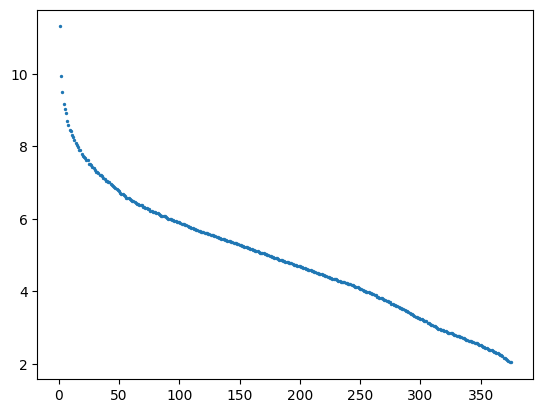
\includegraphics[width=8cm]{./figures/5.3a.png}
    \end{center}

    \textbf{(b)}
\begin{lstlisting} [language=python]
def compress (image, k):
"""
Perform SVD and truncate it, using k singular values/vectors

Params:
image (np.array)

k (int): approximation rank

Returns:
reconst_matrix: reconstructed matrix (tensor in colourful case)

s (np.array): array of singular values
"""
reconst_matrix = []
s = []
if (image.ndim == 2):
    print("BW image")
    U, S, Vt = np.linalg.svd(image)
    V = Vt.T
    Uk = U[:, :k]
    Sk = S[:k]
    Vk = V[:, :k]
    reconst_matrix = Uk @ np.diag(Sk) @ Vk.T
    s = Sk
elif (image.ndim == 3):
    r, g, b = image[:, :, 0], image[:, :, 1], image[:, :, 2]
    
    U, S, Vt = np.linalg.svd(r)
    V = Vt.T
    rr = U[:, :k] @ np.diag(S[:k]) @ V[:, :k].T
    rr = rr.astype(np.int32)
    s.append(S[:k])
    
    U, S, Vt = np.linalg.svd(g)
    V = Vt.T
    rg = U[:, :k] @ np.diag(S[:k]) @ V[:, :k].T
    rg = rg.astype(np.int32)
    s.append(S[:k])
    
    
    U, S, Vt = np.linalg.svd(b)
    V = Vt.T
    rb = U[:, :k] @ np.diag(S[:k]) @ V[:, :k].T
    rb = rb.astype(np.int32)
    s.append(S[:k])

    s = np.array(s).flatten()
    reconst_matrix = np.dstack((rr, rg, rb))

return reconst_matrix, s

figure = plt.figure(figsize=(9, 20))
ax1 = figure.add_subplot(131)
ax2 = figure.add_subplot(132)
ax3 = figure.add_subplot(133)
img5, s5 = compress(img, 5)
img20, s20 = compress(img, 20)
img50, s50 = compress(img, 50)

ax1.imshow(img5)
ax1.set_title('k=5')
ax2.imshow(img20)
ax2.set_title('k=20')
ax3.imshow(img50)
ax3.set_title('k=50')
\end{lstlisting}
which plots
    \begin{center}
        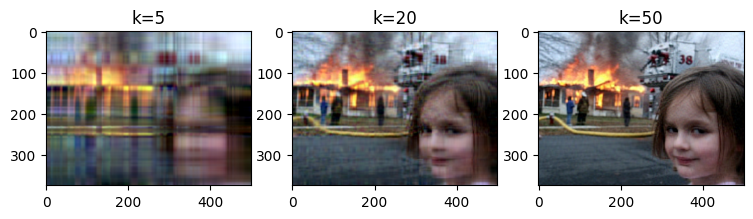
\includegraphics[width=13cm]{./figures/5.3b.png}
    \end{center}


    \textbf{(c)(i, ii)} Working only on the first channel.
\begin{lstlisting} [language=python]
X = img[:, :, 0]

n, p = X.shape
k_vals = np.arange(5, 300, 1)
err_k = np.zeros(k_vals.shape)
U, S, Vt = np.linalg.svd(X)
V = Vt.T

for i, k in enumerate(k_vals):
    Uk = U[:, :k]
    Sk = S[:k]
    Vk = V[:, :k]
    Xhat = Uk @ np.diag(Sk) @ Vk.T
    err_k[i]= np.linalg.norm(X - Xhat)/np.linalg.norm(X)
    
figure = plt.figure()
ax1 = figure.add_subplot(121)
ax2 = figure.add_subplot(122)
ax1.plot(k_vals, err_k)
ax2.plot(k_vals, ((n + p + 1) * k_vals)/(n * p))
\end{lstlisting}
    \begin{center}
        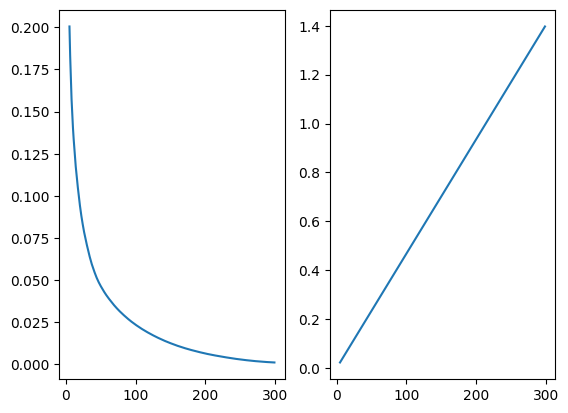
\includegraphics[width=13cm]{./figures/5.3c.png}
    \end{center}
    For a certain $k$, the compression stores $n \times k + k + k \times p = (n + p + 1)k$.
    
    The relative error decreases and plateaus similar to $1/k$ as $k$ increases, while the compression rate increases linearly as $k$ increases. I would choose $k = 150$, to still get around 0.6 compression rate, while keeping relative error relatively low (after the drastic slope in the beginning).
\end{solution}
\end{document}